\chapter{Introduction}
\section{Instability of Plasma Flow}
The instability of plasma flow refers to the tendency of a plasma system to deviate from a stable, equilibrium state and exhibit perturbations or fluctuations in its behavior. A mechanical analogy is shown in Fig.\ref{fig:stability-visualization}. These instabilities can arise from various factors, such as the interaction of particles with electromagnetic fields, collective effects, or the presence of gradients in plasma parameters.

To study instability of a configuration, one can linearize the equations of motion for small deviations from an equilibrium state. \cite{chen_introduction_2016} By assuming the perturbations are oscillatory, meaning that it is proportional to $\exp(-i\omega t)$ and substituting into the linearized equations, one obtains the equations about the frequency $\omega$. Solving for $\omega$ we can examine the instability of of the problem.
\begin{itemize}
  \item If the frequency has positive imaginary part, $\Im(\omega)>0$, the plasma flow is unstable since the perturbed quantities grows exponentially in time, $\exp(\Im(\omega)t)$.
  \item If the frequency has negative imaginary part, $\Im(\omega)<0$, the plasma flow is stable since the perturbations decays over time.

  \item If $\Im(\omega) = 0$, then the plasma flow is also stable. 
\end{itemize}

Therefore, the imaginary part of $\omega$, $\Im(\omega)$, is often called growth rate of instability.

\begin{figure}[htbp]
	\centering
	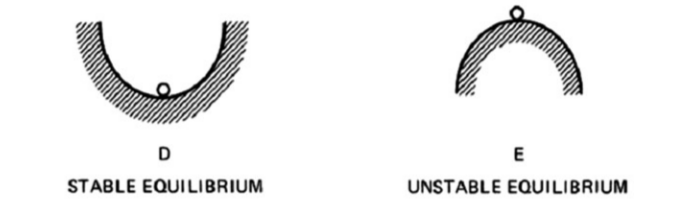
\includegraphics[width=0.7\linewidth]{figures/stability-visualization}
	\caption{Mechanical analogy of various types of equilibrium. Adapted from \cite{chen_introduction_2016}. }
	\label{fig:stability-visualization}
\end{figure}

Plasma flow in magnetic mirror configurations have been studied extensively in plasma physics due to its frequent precense in many areas such as the accretion flow \cite{jockers_stability_1968,aikawa_stability_1979}, and magnetic nozzle\cite{smolyakov_quasineutral_2021}. However, the stability of these configurations remains a debatable subject.

\section{Flow in Magnetic Nozzle}
A magnetic nozzle is a device that uses a magnetic field to shape and control the flow of charged particles in a plasma propulsion system, see Fig.\ref{fig:magnetic-nozzle}. By employing the magnetic mirror configuration, the magnetic nozzle can effciently direct and accelerate the plasma flow, generating thrust for propulsion. The magnetic field in the nozzle helps collimate and focus the plasma exhast, increasing its velocity and enhancing the performance of the propulsion system.

\begin{figure}[htbp]
  \centering
  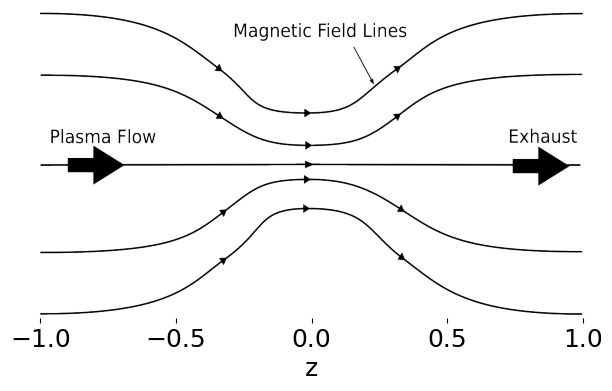
\includegraphics[width=0.7\linewidth]{figures/magnetic-nozzle}
  \caption{A simplified model of the magnetic nozzle}
  \label{fig:magnetic-nozzle}
\end{figure}

\subsection{Magnetic Field in Magnetic Nozzle}
In 1D problem, the magnetic field can be modeled as
\[ B(z) = B_0 \left[1 + R\exp(-\left(\frac{x}{\delta}\right)^2)\right] \]
where $1+R$ is the magnetic mirror ratio, and $\delta$ determines the spread of the magnetic field. It is shown in Fig.(\ref{fig:magnetic-field}).
\begin{figure}[H]
	\centering
	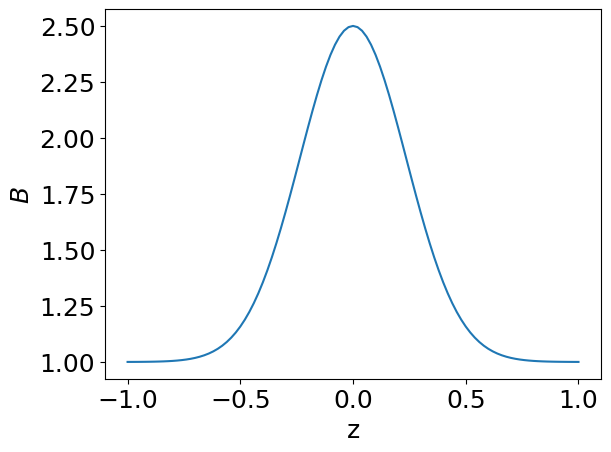
\includegraphics[width=0.7\linewidth]{figures/magnetic-field}
	\caption{This is the magnetic field in nozzle with mirror ratio $1+R=B_{max}/B_{min}=2.5$, and the spread of magnetic field, $\delta=0.1/0.3=0.\bar{3}$. }
	\label{fig:magnetic-field}
\end{figure}

\section{Governing Equations for Flow in Magnetic Nozzle}
In this section, we will derive the governing equations of the flow in magnetic nozzle, starting from the fluid description for plasma.

In magnetic nozzle, the magnetic field is along the nozzle, which we denote as z-axis. Due to Lorentz force, the charged particles gyrates about the magnetic field lines. Because the magnetic moment is invariant in such situation (\textbf{reference}). The fluid velocity of particles can be written as $\mathbf{v} = v\mathbf{B}/B$, meaning that the particles move along the magnetic field lines. Therefore the conservation of density 
\[ 
\pdv{n}{t} + \div(n\mathbf{v}) = 0 
\Rightarrow 
\pdv{n}{t} + B\pdv{z}(\frac{nv}{B}) = 0  
\]
In the derivation, $\div{\mathbf{B}} = 0$ is used.

To derive the second governing equation, we start from the conservation of momentum, 
\[ \pdv{v}{t} + v\pdv{v}{z} = -\frac{1}{\rho}\grad{p} \]
Let $\grad{p} = k_BT\pdv*{n}{z}$, we have
\[ \pdv{v}{t} + v\pdv{v}{z} = -c_s^2\frac{1}{n}\pdv{n}{z} \]
where $c_s^2 = k_BT/m$ is the square of sound speed.

Therefore the dynamics of the flow in magnetic nozzle can be characterized by the conservation of density and momentum,
\begin{align} 
	&\pdv{n}{t} + B\pdv{z}(\frac{nv}{B}) = 0\label{eq:conservation-of-density}\\ 
  &\pdv{v}{t} + v\pdv{v}{z} = -c_s^2\frac{1}{n}\pdv{n}{z} \label{eq:conservation-of-momentum}
\end{align}

\subsection{Velocity Profile at Equilibrium}
Let $n_0$ and $v_0$ be the density and velocity at equilibrium (stationary solution). Substitute them into Eq.(\ref{eq:conservation-of-density}) and Eq.(\ref{eq:conservation-of-momentum}), we get the so-called equilibrium condition which $n_0$ and $v_0$ must satisfy,
\begin{align*}
	&\pdv{z}(\frac{n_0v_0}{B}) = 0 \\
	&v_0\pdv{v_0}{z} = -c_s^2\frac{1}{n_0}\pdv{n_0}{z} 
\end{align*}

Let $M(z) = v_0(z)/c_s$ be the Mach number (nondimensionalized velocity). We can express $M$ using the Lambert W function,
\[ 
M(z) = \left[ -W_k\left(-\frac{B(z)^2}{B_m^2}M_m^2e^{-M_m^2}\right) \right]^{1/2} 
\]
where the subscript $k$ of $W$ stands for branch of Lambert W function. When $k=0$, it is the subsonic branch; When $k=-1$, it is the supersonic branch. Below shows a few cases of the solution.
\begin{itemize}
	\item $M_m < 1, k=0$, subsonic velocity profile.
	\item $M_m = 1$, $k=0$ for $x<0$ and $k=-1$ for $x>0$, accelerating profile
	\item $M_m = 1$, $k=-1$ for $x<0$ and $k=0$ for $x>0$, decelerating profile
	\item $M_m > 1, k=-1$, supersonic velocity profile
\end{itemize}
 Fig.(\ref{fig:velocity_profiles}) shows some cases of the solution.
\begin{figure}[H]
	\centering
	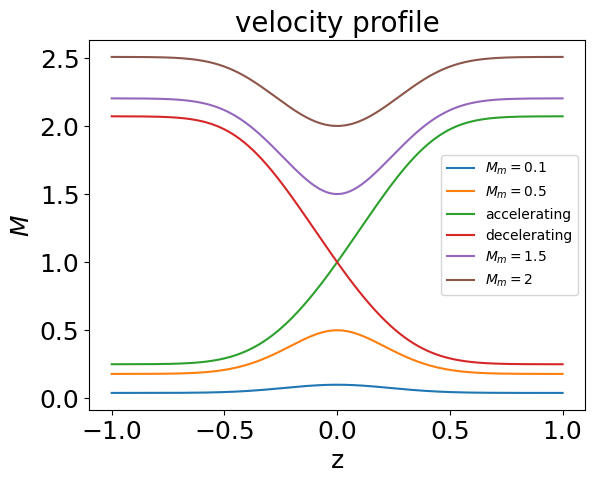
\includegraphics[width=0.7\linewidth]{figures/velocity-profiles}
	\caption{The velocity profile in the magnetic nozzle is completely determined by $M_m$, the velocity at the midpoint, $z=0$. For the transonic velocity profiles, $M_m$ alone is not enough to determine the profile, we need to specify the branch of Lambert W function to determine whether it is accelerating or decelerating.}
	\label{fig:velocity_profiles}
\end{figure}

\section{Linearized Equations}
For convenience, we nondimensionalize the governing equations by normalizing the velocity to $c_s$, $v\mapsto v/c_s$, $z$ to system length $L$, $z \mapsto z/L$ and time $t\mapsto c_s t/L$. The governing equations become
\begin{align}
    &\pdv{n}{t} + n\pdv{v}{z} + v\pdv{n}{z} - nv\frac{\partial_z B}{B} = 0 \\
    &n\pdv{v}{t} + nv\pdv{v}{z} = -\pdv{n}{z}
\end{align}
and the nondimensionalized equilibrium condition is
\begin{align}
    &\pdv{z}(\frac{n_0v_0}{B}) = 0 \label{eq:equilibrium-convervation-of-density}\\
    &v_0\pdv{v_0}{z} = -\frac{1}{n_0}\pdv{n_0}{z} \label{eq:equilibrium-convervation-of-momentum}
\end{align}

Now we are going to derive an important intermediate result, the linearized governing equations.
    Let $n = n_0(z) + \tilde{n}(z,t)$ and $v = v_0(z) + \tilde{v}(z,t)$, where $\tilde{n}$ and $\tilde{v}$ are small perturbed quantities. The linearized governing equations are
  \begin{align}
      &\frac{1}{n_0}\pdv{\tilde{n}}{t} 
      + \pdv{\tilde{v}}{z} + v_0\tilde{Y} + \tilde{v}\frac{\partial_z n_0}{n_0} - \tilde{v}\frac{\partial_z B}{B} = 0 
      \label{eq:linearized-conservation-of-density}
      \\
      &\pdv{\tilde{v}}{t} + \pdv{(v_0\tilde{v})}{z} = -\tilde{Y}
      \label{eq:linearized-conservation-of-momentum}
  \end{align}
  where 
  \[ \tilde{Y} \equiv \frac{1}{n_0}\pdv{\tilde{n}}{z} - \frac{\partial_z n_0}{n_0^2}\tilde{n} = \pdv{z}(\frac{\tilde{n}}{n_0}) \]

\section{Polynomial Eigenvalue Problem}
In order to investigate the instability of magnetic nozzle, we need formulate it as an eigenvalue problem. To do that, we assume the perturbed density and velocity are oscillatory, i.e. $\tilde{n}, \tilde{v} \sim \exp(-i\omega t)$, where $\omega$ is the oscillation frequency of the perturbed quantities. This frequency can be a complex number. If $\omega = \omega_r +i \omega_i$, then the perturbed quantities becomes $\tilde{n} \sim \exp(\omega_i t)\exp(i\omega_r t)$, which means it grows exponentially with time.

Let $\tilde{n}\sim \exp(-i\omega t)$ and $\tilde{v} \sim \exp(-i\omega t)$, then we have the polynomial eigenvalue problem
\begin{equation}
  \begin{aligned}
    &\omega^2 \tilde{v} \\
    +& 2i\omega\left(v_0\pdv{}{z} + \pdv{v_0}{z}\right) \tilde{v} \\
    +& \left[ (1-v_0^2)\pdv[2]{}{z} 
      -\left(3v_0 + \frac{1}{v_0}\right)\pdv{v_0}{z}\pdv{}{z} 
      -\left(1-\frac{1}{v_0^2}\right)\left(\pdv{v_0}{z}\right)^2 
    - \left(v_0+\frac{1}{v_0}\right)\pdv[2]{v_0}{z} \right]\tilde{v}
    = 0
  \end{aligned}
  \label{eq:polynomial-eigenvalue-problem}
\end{equation}

% \subsection{Flow in Similar Configuration: Bondi-Parker Flow}
% Bondi derived a steady-state solution for accretion flow which is governed by Bernoulli's equation in sperical symmetry around a point mass in 1952. Then Parker solved a similar problem but with outward wind in 1958. \cite{aikawa_stability_1979,bondi_spherically_1952,keto_stability_2020} The equilibrium velocity profiles in such configuration are shown in Fig.\ref{fig:BP-flow-velocity}.

% \begin{figure}[htbp]
%     \centering
%     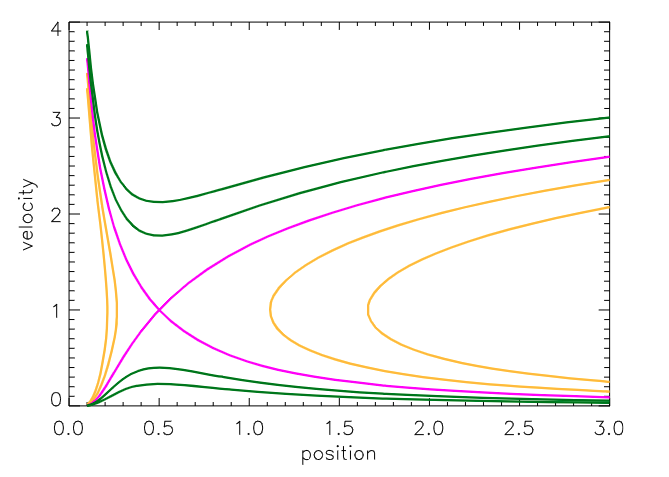
\includegraphics[width=0.7\textwidth]{figures/steady-state-BP-flow}
%     \caption{Representative trajectories of the steady-state BP flow in non-dimensional units. \cite{keto_stability_2020} The upward pink line represents a outward wind, it accelerates from subsonic to supersonic. The downward pink line represents an accretion flow, it accelerates towards the mass point. The green lines below the pink lines represent subsonic flows, and the green lines above represent supersonic flows. Orange lines are physically impossible scenarios.}
%     \label{fig:BP-flow-velocity}
% \end{figure}

% Solar wind is an example of Bondi-Parker flow. The solar wind is a stream of charged particles, primarily electrons and protons, flowing outward from the Sun. 


\section{Goal of this Thesis}
The goal of this thesis is to study the instabilities of the magnetic mirror configuration given certain boundary conditions and equilibrium velocity profiles.

To achieve the goal, first we need to study the spectral method for solving the instability problem. To use spectral method, it is necessary to understand different discretizations of the operators, such as finite difference, finite element and spectral element method.

Once the spectral method is introduced, we can use it to study the instability of plasma flow in magnetic nozzle as an eigenvalue problem. We can obtain results by using different discretization techniques. By comparing the results from different approach, we can increase the credibility of the true solution.

However, spectral method is not suitable when the equilibrium velocity profile is transonic due to the precense of singularity at the sonic point. We need to solve the singular perturbation problem around the singularity analytically. Then starting from the singular point, we can use shooting method to find eigenvalues.

